\chapter{Literature Review}
\label{chap:related_works}


\section{Data Mining}

Data collection from some original source provides access to a data set that may not be initially available. This data source could also be in a state that is not convenient or feasible for use without leveraging data mining techniques to transform the data to a more accessible state. The source of the data can vary greatly based on the interests for the individual(s) collecting the data. Data mining has mostly focused on single source mining and multiple data sources. Data mining in general has however also taken a large focus on data collection from software repositories which can be either single or multiple source \cite{Hemmati2013}, \cite{Hassan2006}, ... %TODO list other msr based papers.
% TODO find other work of data mining

% MSR, guiding future changes
Zimmermann et al. map the changes that certain developers make and who change certain functions to the functions they also change \cite{Zimmermann2005a}. 

% Change analysis
Maletic and Collard investigate changes with a software project's development cycle. The changes are extracted and stored in an more easily usable representation \cite{Maletic2004}.

% MSR Change extraction of changes
Canfora et al. propose a method for extracting and refining the changes made throughout the life a project to be used in more effective analyses \cite{Canfora2007c}.

Hemmati et al. take a comprehensive look at the research related to \gls{msr} to determine best practices and point towards future work \cite{Hemmati2013}.

% MSR in general
Hassan cover the different metrics and uses of \gls{msr} \cite{Hassan2006}.

% Validation of Change history research, benchmark
Dit et al. provide a benchmark dataset to help in the testing and comparing of various methods for improving software maintenance tasks \cite{Dit2013}.

% TODO MERGE this with related work
\subsection{Mining Open Source Software Repositories}

% TODO ensure this is accurate.
\gls{oss} generally is software that provides with the ability access the source code and make modifications to the source code. While certain licenses provide some restrictions on the ability to redistribute the software the main point of the source code of the software being freely available is key. The scope and capability of \gls{oss} projects vary greatly. Several very popular \gls{oss} projects are listed in table \ref{tab:oss_projects}.

%TODO make sure footnotes fit in better.
\begin{table}[h!]
\begin{minipage}{\textwidth}
\begin{center}
    \begin{tabular}{|l|l|l|}
        \hline
        Owner & Project & Description \\
        \hline
        Mozilla & Firefox\footnote{\url{https://www.mozilla.org/en-US/firefox/desktop/}} & Internet Browser \\
        Linux & Linux Kernel\footnote{\url{https://www.kernel.org/}} & Operation System Kernel \\
        VideoLAN & VLC\footnote{\url{http://www.videolan.org/vlc/index.html}} & Media Player \\
        PostgreSQL & PostgreSQL\footnote{\url{http://www.postgresql.org/}} & Object-Relational Database Management System \\
        git & git\footnote{\url{https://git-scm.com/}} & Version Control System \\
        \hline
    \end{tabular}
\end{center}
\caption{Open Source Software Projects}
\label{tab:oss_projects}
\end{minipage}
\end{table}
%Firefox => MPL 2.0
%Linux Kernel => GPL v2, plus various closed-source binary blobs
%VLC => GPLv2+ (player), LGPLv2.1+ (engine)
%PostgreSQL => PostgreSQL License
%git => GNU General Public License v2, GNU Lesser General Public License 2.1

The development of large software projects (whether \gls{oss} or not) often make use of \gls{vcs}. A \gls{vcs} helps the developers of the project manage the changes of the project and facilitate the collaboration between developers. A \gls{vcs} will keep an current version of the project and keep track of the previous version of the project as well. This may be done through keeping a copy of each version of the project or by keeping track of all each change made to the project. \gls{svn} and git would be two examples of \gls{vcs}s.

Git is a \gls{dvcs} and differs greatly from \gls{svn} which is a normal \gls{vcs}. Git will provide the user with a complete copy of the repository that is worked on independent of network connection. The independence of each repository also allows for a repository to be developed without a centralized server. The distributed aspect of git tends to allows for easier use for all involved parities. The one main issue with a \gls{dvcs} is that while decentralization is useful, developers will require some method to collaborate and communicate to transfer changes made to the repository. Therefore typically one centralized server is used to maintain communication between all interested parties.

Git has grown in popularity since it was created and is at the core of several \gls{vcm} sites such as GitHub \footnote{\url{https://github.com/}}, BitBucket \footnote{\url{https://bitbucket.org/}} and GitLab \footnote{\url{https://gitlab.com/}}. These platforms tend to be fairly supportive of \gls{oss} projects through providing their services free of charge. For example, GitHub provides unlimited public repositories completely free. While these projects do not have to be licensed with an open source license typically they will be since they are already publicly visible.

% GitLab -> https://gitlab.com/
% GitHub -> https://github.com/
% BitBucket -> https://bitbucket.org/

GitHub is the most popular of the \gls{vcm} websites and hosts numerous very popular \gls{oss} projects including, the Linus Kernel, Swift\footnote{\url{https://swift.org/}} and React\footnote{\url{https://facebook.github.io/react/}}. GitHub also provides a public \gls{api} to allow for access to the data related to project repositories which is discussed further below. % TODO link to that.
Given the popularity of GitHub for use by developers and the availability of the project data, GitHub is an obvious choice for mining project data. Especially since the goal of mining software is to capture \gls{oss} project data to both explore and test analysis methods. Publicly visible projects are also publicly accessible through the \gls{api} and the majority are open source.

%%%%%%%%%%

Git provides a simple interface to manage the repository regardless of which site is the central server. Therefore regardless which site the project resides on users can easily interact with the project as long as they know the git interface. Git in essences is a file storage for the project that keeps track of changes made to the project. A \textit{commit} is a set of changes that a developer has made at a certain time. The developer has full control what gets committed, when it gets committed and even modified at a later date.
%This results in the date of the commit merely identifying when the developer formally notified Git that a change was made.

A branch is a series of commits that are often related. In figure \ref{fig:network_diagram}, each dot would represent a commit and a set of dots connected by the same colored lines are a branch. Branches can be considered different paths or deviations in the development from each other allowing for different versions of the project to be maintained and developed. The \textit{master} branch is the main branch, represented with black, from which all branches usually stem from and is generally where projects are developed on. On a similar note, a \textit{tag} is a branch that is frozen to allow for future reference. Tags are often uses to mark a significant point in the development history such as a project release. Finally, when two differently branches converge into a single dot then the two branches have been \textit{merged}. A merge indicates that the differences between the two branches are consolidated based on the developer's discretion.

\begin{figure}[!ht]
    \centering
        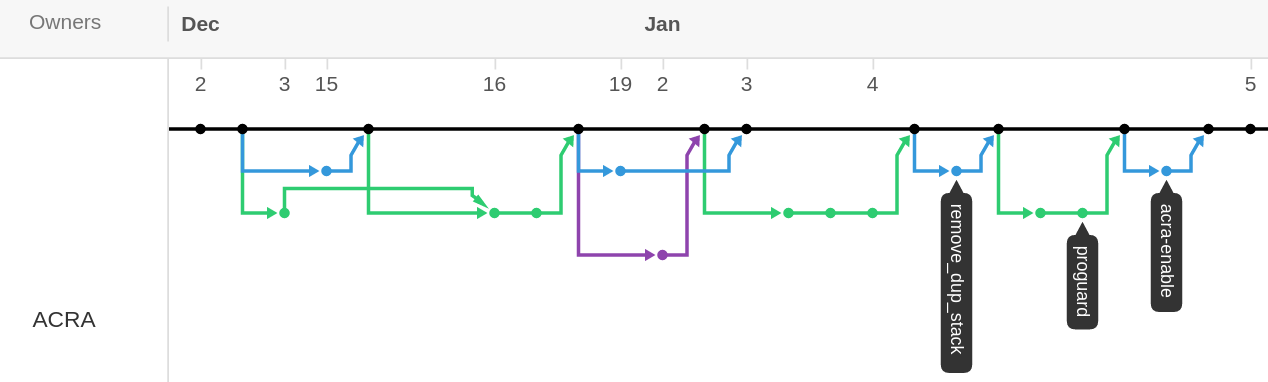
\includegraphics[width=1.0\textwidth]{images/network}
    \caption{Network diagrams}
    \label{fig:network_diagram}
\end{figure}

A commit consists of files that have been changed, more specifically a list of \textit{patch} files which each outline the changes made to their corresponding file. The patch file consists of a series of differences between the previous version of the file and this new version of the file. These patch files are key since they contain the actual changes made to the project and thus are the major point of interest.

% TODO fix close

\section{Machine Learning}

% Rase, realizing software engineering learning
Machine learning is a complex method for software algorithms to attempt to determine patterns within the data. One such problem example would be an algorithm to detect certain people within an image. For an individual such a task may seem trivial however for a software system to detect it is far more difficult. Algorithms that can determine patterns and mimic them from abstract set of data is useful when such patterns are extremely complex. There are numerous algorithms which apply machine learning approaches. Each approach has both advantages or disadvantages. Some examples of machine learning algorithms are \gls{svm}, \gls{rf} and \gls{ann}. The three provided examples are also commonly used for data mining \cite{Alam2013}, \cite{Granitto2007}, \cite{Westland2011}, \cite{Yu2011}, \cite{Huang2007}, \cite{Jalbert2012} %TODO get some papers for svm and ann

Bhattacharyya et al. provide a detailed description of \gls{rf} and \gls{svm}.

\subsection{Support Vector Machines}
\label{subsec:svm_prediction}

\gls{svm} models are more easily modified to fit data from different sources since they flexible and robust than more classical linear regression models *cite*. %TODO consider citing 

A \gls{svm} is used to predict what type of change will occur based on a set of features provided. A feature is a data extracted from the project represented as a floating point number. In order to be useful a feature must in some way characterize the the category that it is assigned to. The feature must also not rely on the category that it belongs to in order to be calculated. For example, given a category of the method change within the next 5 commits or not, then the features must not rely on knowledge of future changes to the project. If the features fail to effectively characterize the category they are assigned to then the \gls{svm} may have poor predictions. It is also necessary for the features to independent of each other to not negatively affect the categorization.


\gls{svm} has been widely used for making predictions for various aspects including predicting battery charge state \cite{Anton2013}, pharmaceutical data \cite{Burbidge2001}, software faults \cite{Gondra2008, Erturk2015, Malhotra2015, Kim2008, Moeyersoms2015, Neuhaus2007}, bug localization \cite{Murphy2007, Neuhaus2007}, software mutation testing score \cite{Jalbert2012}, financial stocks \cite{Kim2003}, credit score \cite{Huang2007}, credit card fraud \cite{Westland2011}, solar power output \cite{Zeng2016}.

Malhotra reviews numerous machine learning techniques, including \gls{svm} and \gls{rf}, used by various studies. The results of which outline where each approaches succeed and falls short. When using a machine learning algorithm it is imperative to use a suitable algorithm for current situation. Kim et al. outline a approach that uses a \gls{svm} to predict changes that will occur within the project. By identifying these changes the a project developer can potentially locate a bug within a change and fix it prior to being reported. Erturk and Sezer compare the performance of their proposed method, an Adaptive Neuro Fuzzy Inference System, to that of an \gls{svm} for predicting software faults. The models are trained using project metrics as well as the project's historical fault data. Zeng and Qiao use a \gls{svm} to provide short-term predict solar power output. The \gls{svm} model outperformed both an autoregressive and a neural network model. Anton et al. propose a method for predicting the state of charge of a battery using \gls{svm} model.

Bhattacharyya et al. uses \gls{rf}, \gls{svm}, logistic regression to detect credit card fraud. Both \gls{rf} and \gls{svm} are able to predict a large number of fraudulent credit card transactions.


% TODO talk even more about how to pick better features.
%<<< TODO Example feature vector >>>

% \begin{table}
% \begin{center}
%     \begin{tabular}{|l l l l l l l|l|}
%         \hline
        
%         Features &  &  &  &  &  &  & Description \\
%         \hline
%         $name$ & $signature$ & $change_i$ & $committer$ & $freq_{change}$ & $change_{prev}$ & $t_\Delta$ & $change_{next\_6}$ \\
%         %0.0 & 0.1 & 0.0\\
%         \hline
%     \end{tabular}
% \end{center}
% \caption{Example Feature Vector}
% \label{tab:example_feature_vector}
% \end{table}

% TODO Format parts of this.
\gls{svm} requires all feature data be encoded as floating point numbers. For any numerical data the conversion to floating point is trivial. However, for more complex data the conversion is a little more difficult. Categorical data can be mapped into a unique vector entry per category. For example, if a feature can be 1 of 3 options: 0, 1 or 2 then it can be converted into three entries in the feature vector. Encoding the value 2 the sub-vector of the feature set would be [0, 0, 1] where 1 indicates a field that feature is present in the data for this vector, and 0 indicates the feature is not present. Data that is in the form of a string can be converted to a floating point number by assigning a unique number for each string (similar to hashing). The one downside to this method is that the numbers corresponding to each string maintain no numerical properties. In essence the data becomes categorical, such that if \textit{bob} is mapped to 1 and \textit{sally} is mapped to 2 there is no relationship between 1 and 2. Ideally, this data would then be further converted using the previously described method however if the set of possible strings is large then it may be unreasonable to convert it. For example, if there are 100 possible strings then that would add 100 new entries to a single vector.

%<<< TODO svm diagrams >>>

The categorization is used for the prediction, where each value of the category relates to a unique prediction type. For example, a simple binary categorization could simply 1 or 0 where 1 predicts the event will occur and 0 predicts that the event will not occur. In essence an \gls{svm} is tasked with separating a dataset into two different categories given a sample set of data that has already been categorized into two subsets. Given the categorization of the sample dataset the \gls{svm} model is trained to allow for categorization of new data. The categorization of any new vectors (that were not used for training) is called a prediction and is made by the \gls{svm} model created through the training. More specifically, the sample dataset is a dataset extracted from the target dataset. The sample dataset is then categorized based on the predetermined criteria (the prediction goal). This dataset along with the categorization for each vector in the dataset is the training dataset, and is then used to \textit{train} the \gls{svm} model. Once the model has been trained, the \gls{svm} model is ready to be used for making classification predictions. The data for each feature can be extracted from the new dataset, allowing for the model to classify each new vector. Given that the \gls{svm} model is accurate and reliable the results can then be used towards making predictions about the dataset. For example if the classification is that of predicting change to occur within the next six commits the developer may wish to be careful with the use of the method or assess the method's quality and determine if any issues within the method need to be addressed.

A lower prediction score often relates to the data from the feature set poorly characterizing the categories. Similarly a warning will be given if the dataset is in-separate. In this case, the dataset for each category may be too similar and cannot be properly split into the two category subsets. In both cases a change to the feature set may help, whether that is a decrease or increase of features in the set. Some features are detrimental to the model, especially two features related to one another. Other potential steps would be to modify the data to ...
% *** TODO determine best practices for data something like mean of 1 and std of 1. ***

More details about the specific features used will be given a little later on. Features are descriptive aspects of the dataset that are classified into the predetermined categories. Since these features relate directly to the category understanding of the classification critical and can help determine which features should be used. For example for a classification of whether a change will occur within the next few commits, a useful feature may be the frequency by which a method changes within the project. Picking a descriptive feature set is paramount to providing a strong prediction of future data.

%<<< TODO create a figure to outline the various features and their meaning >>>

Most of this was done using database queries or user defined functions created in the database language.

% TODO get some papers related to support vector machines.

\subsection{Random Forests}
\label{subsec:random_forest_predictions}

\gls{rf} are a popular machine learning algorithm and is used in numerous areas including predictions for software fault \cite{Malhotra2015, Moeyersoms2015, Guo2004}, software development effort \cite{Moeyersoms2015}, credit card fraud \cite{Westland2011}, database indexing \cite{Yu2011}, malware detection \cite{Alam2013}. 

Malhotra provides an extensive review of studies involving machine learning to predict software faults. The results showed that \gls{rf} tended to preform better than other machine learning algorithms studied. Moeyersoms et al. made use of \gls{rf} and \gls{svm} as well as a few other data mining approaches to predict software faults and effort estimation. The data mining techniques are used as part of another model, ALPA rule extraction, to improve the predictions and increase traceability. Guo et al. attempt use \gls{rf} to predict the fault proneness of modules within a project. The \gls{rf} prediction results for the five sample projects prove more accurate to that of a logistic regression. Yu et al. attempt to use \gls{rf} to determine a more effective database indexing for video data. The database index are used to provide faster searching of the database for action detection.

\gls{rf}s are commonly used to on data that has been mined from some source to make predictions \cite{Alam2013}, \cite{Granitto2007}, \cite{Yu2011}. A \gls{rf} leverages numerous decision trees to provide attempt to improve prediction capabilities. Therefore to fully understand a \gls{rf} first an understanding of decision trees is necessary. A decision tree is a technique which will create a tree based on a data set that has been classified. Once the decision tree model is created it can be used to predict or categorize data that has not yet to be classified. In the tree model the leafs will be categorizations where as the connections between inner nodes are the decisions by which the categorizations are made.

% TODO format
One issue with decisions trees and more generally machine learning techniques in general is imbalanced data sets for training the model \cite{Khoshgoftaar2007}. The data set used rarely provided even sample sizes of each set therefore without taking necessary pro-cautions the algorithm will bias the results. In the worse case the model will classify any input data as the larger data classification.

In case of imbalanced datasets there are several methods to help provide stronger predictions \cite{Khoshgoftaar2007}. The most obvious and easiest to attempt would be to sample more data. However if the dataset in general follows this trend then some more advanced techniques can used to improve the model.

% Note when remarking about model quality this refers to accuracy and recall of the model
 
The first method would be to \textit{undersample} larger category this will even out both of the categories. This will remove some of the input values within the dataset to reduce the set size. However if there are very few samples of the smaller category the performance will suffer as well. A second method of \textit{oversampling} is useful in the case were the data samples are small. The input data from the smaller category is selected to be duplicated in the set to increase the size of the set. This helpful since it will increase the size of the dataset but could lead to bias based on the data selected from the smaller dataset. The selection method for which input vectors to over or under sample can be based off on the data's statistical distribution or made by random choice. Another advantage of these over and under sampling is that they can also be used together to in the case of a large disparity between the category's set size. 

% Bootstrapping aggregation
Another feature of \gls{rf} which is used to help provide more reliable predictions is \textit{Bootstrap Aggregation} \cite{Westland2011}. Similar to normal sampling methods it will take the initial dataset. However rather than using the dataset as is the dataset will be uniformly sampled $n$ times and repeated $m$ times to create $m$ datasets of $n$ values. These newly created datasets will then be used to train $m$ models. Finally, when attempting to categorize a new input data it will be given to every model and the prediction result will be aggregated to provide a more accurate results. For some machine learning methods such as \gls{svm} this method will improve the results and help with imbalanced datasets.

A \gls{rf} is a collection of decisions trees trained on random samples of the initial dataset. So the \gls{rf} will take an input dataset and then train $m$ decisions trees using $m$ randomly sampled sub-datasets of the initial dataset. This helps improve the model created and makes \gls{rf}s far easier to use. As well \gls{rf}s have a feature that determines the importance of each feature is assessed during the training of the model \cite{Westland2011}. The importance outlines the quality of each feature in providing the prediction \cite{Verikas2011}. Therefore in order to properly understand the feature importance the accuracy, precision and recall of the model should be determined by running a test dataset to determine the quality of the model.

\section{Software Development Prediction}
% TODO actually write about each of the papers.

%TODO work this together 
Software development prediction contains numerous areas of study which generally attempt to improve projects by focusing on their development and providing feedback to the developers through predictions. Some of these areas include, fault detection \cite{Nagappan2007, Moser2008, Thwin2005, Sisman2012}, mutation score \cite{Jalbert2012}. While there may be a large overlap in the objective for these studies often they will vary in what is used to make the prediction.

% Close source, prediction
%Nagappan and Ball use the software dependencies and churn metrics to predict the failure of a commercial product post release \cite{Nagappan2007}.

% Defect prediction, change attributes, static attributes
%Change and static code attributes are compared in their capability in predicting defects within a project \cite{Moser2008}.

% predict software quality based on code metrics
%Attempt to predict the number of defects within a given class using a neural network trained on object oriented code metrics \cite{Thwin2005}. Second the amount of changes within a class is predicted again with a neural network using object oriented code metrics \cite{Thwin2005}.

% Prediction of something
%Support development of software predictions is a common research area. Jalbert and Bradbury used static metrics from both the source code and corresponding test suites to predict the mutation score for the test suite \cite{Jalbert2012}.

% Bug localization through prediction, change history, defect history, temporal decay.
%Sisman and Kak leverage defect history and the change history of a project to predict which files will be the cause of bugs in different version of the project \cite{Sisman2012}.

\subsection{Change Prediction}
% Related work stuff here or later

The development of large scale projects can take a long time and involve a huge time investment from the developers. The development of the project will cause for the developers to make changes to projects. Software projects will have faults within the project especially during the development phase. A project in its early stages may not meet the full set of functionality since it has not been completed yet. Since the development team will known that such features are not yet implemented these faults or fails are not a huge concern. Rather faults that are unknown to the developer team are far more serious. Such cases as a feature was thought to be implemented correct but was not or a feature implementation breaks other features. In both those cases changes made to the project cause the fault to be revealed.

Changes to the project are the means by which all development occurs. The ability to analyze and predict changes within a project could give deep insights into the development of a project.


A large amount of research as focused on predictions of changes based on changes \cite{Bantelay2013}, \cite{Chaturvedi2014}, \cite{Giger2012}, \cite{Hassan2004}, \cite{Kagdi2007}, \cite{Ying2004}. 

Ying et al. present a method that predicts which parts of the system will change given a set of changes \cite{Ying2004}. The prediction method leverages the change history.

Kagdi and Maletic also leverage version history changes to perform software change predictions \cite{Kagdi2007}. The actually analysis applied is two fold, through the dependency analysis of the current version and the change analysis of the version history. The data is collected through \gls{msr} which is a popular field of study. 

In a similar work, Hassan and Holt, worked towards predicting change propagation of a given initial change. \cite{Hassan2004} The main question was to determine given a change to an entity (e.g. function or variable) will propagate to changes in other entities. This work is very related since it tests various methods and leverages presents the best one.

Bantelay et al. propose a method that mines the file and method level evolutionary couplings to attempt to predict commits and other interactions within the project \cite{Bantelay2013}. Both methods were used in isolation as well to determine whether the attributes were more helpful when used together.

Giger et al. attempt to build off of previous work in change prediction (proneness) by providing predictions relating to more refined entities \cite{Giger2012}. The syntax changes are recorded but an attempt is made to capture semantic changes on the statement level \cite{Giger2012}.

Chaturvedi et al. attempt to predict the complexity of the project given it's change history using an entropy analysis \cite{Chaturvedi2014}.

% Change prediction (proneness), visualization
Further work in change analysis was done by Bieman et al. in studying the change-proneness of different entities within a software project \cite{Bieman2003}. In order to provide a deeper understanding visualizations were used as well providing a bit of a different approach from some of the other works.

% Change prediction (proneness)
Koru and Liu study and describe change-prone classes found within open source projects \cite{GunesKoru2007}.

% impact of changes aka precursor to predicting changes. Providing a type of rudimentary prediction by taxonomy.
Wilkerson attempts to classify different types of changes that occur to a project throughout its development \cite{Wilkerson2012}. The classification can then be used to identify the impact that a given change will have on other aspects of the project.

% (TODO check) Close source, identifying areas likely to have change
Snipes et al. describe a tool for analyzing software projects to identify areas that have a history of large amount of change. \cite{Snipes2011}






% TODO talk about previous work on change prediction. cause. 

%There are several different areas of study that are related to this work. Some are more closely related than others and will receive more attention accordingly. A quick summary of the fields that are related are as follows: 

% TODO run libsvm analysis on best candidate feature set.

% TODO work on.
% - Data Mining
%   - MSR is a great place for these types of works.
% - Repository/Version History analysis
%   - Analyzing the changes made to the project to some end.
% - Prediction systems
%   - Change prediction
%   - Predicting whether change will occur or which changes will occur given using some data set.

%21/20-25

% Change Prediction, version history as resource

% \begin{table}
% \begin{center}
%     \begin{tabular}{|l|l|l|l|l|l|}
%         \hline
%         Author & AI Technique & Source & Data & Goal & Accuracy \\
%         \hline
%         Ying et al. & N/A - Uses previous changes & CVS & Change Patterns & Related source code that should change & Mozilla: \{ P:50\% R:20\%-30\% \} Eclipse: \{ P:30\% R:10\%-20\% \} \\
%         Kagdi and Maletic & N/A - Impact Analysis & SVN & Current and historical dependencies & Software change & N/A \\
%         Hassan and Holt & Heuristics & CVS and Perforce & Change History & (Varies) Developer Co-Changes and Entity Co-Change and Entity Co-Call Use Define (CUD) and Entity Co-Change File & Accuracy \\
%         \hline
%     \end{tabular}
% \end{center}
% \caption{Experiment projects}
% \label{tab:project_summary}
% \end{table}



% ~ denotes an approximation based on a graph.
%  ** Best performance

% Author & AI Technique & Source & Data & Goal & Accuracy

% Ying et al. & N/A - Uses previous changes & CVS & Change Patterns & Related source code that should change & Mozilla: { Precision: 0.50, Recall: 0.20-0.30} Eclipse: { Precision: 0.30 Recall: 0.10-0.20 }

% Kagdi and Maletic & N/A - Impact Analysis & SVN & Current and historical dependencies & Software change & N/A

% Hassan and Holt & Heuristics & CVS and Perforce & Change History & (Several Methods) Developer Co-Changes (DEV), History Entity Co-Change (HIS), Entity Co-Call Use Define (CUD), Entity Co-Change File (FIL) and Hybrid (HYB) & DEV: {Precision: 0.01, Recall: 0.74 }, HIS { Precision: 0.06, Recall: 0.87 }, CUD { Precision: 0.02, Recall: 0.42}, FIL { Precision: 0.12, Recall: 0.83 }, HYB(80, 10) { Precision: 0.49, Recall: 0.51 }**, HYV(80,30) { Precision: 0.35~, Recall: 0.65~ } HYB(60,30) { Precision: 0.25~, Recall: 0.75~ } & Very Related

% Bantelay et al. & Impact Analysis & Mylyn and CVS & Interactions (through Mylyn) and commit history and relationships (CVS) & Commit Prediction

% Thwin and Quah & Neural Networks (Ward Neural Network and General Regression Neural Network (GRNN)) & Source Code (Static Analysis from Project) & Object Oriented static metrics (inheritance, complexity, cohesion, coupling and memory metrics) & 1: Number of defects in a class, 2: number of lines changed per class & Correlation is tested rather than accuracy. 1: (R^2: 0.88, r: 0.94; R^2: 0.86: r: 0.94) 2: (R^2: 0.71, r: 0.86; R^2: 0.56, 0.76)


% Jalbert & Support Vector Machine & Source Code (Static Analysis from Project) & source code static metrics and test suite static metrics & predict test suite mutation score & approx 0.71
